\documentclass[12pt,twoside]{book}
\usepackage{../../thesis}
\graphicspath{ {../../images/} }
\usetikzlibrary{calc}
\tikzset{
    right angle quadrant/.code={
        \pgfmathsetmacro\quadranta{{1,1,-1,-1}[#1-1]}     % Arrays for selecting quadrant
        \pgfmathsetmacro\quadrantb{{1,-1,-1,1}[#1-1]}},
    right angle quadrant=1, % Make sure it is set, even if not called explicitly
    right angle length/.code={\def\rightanglelength{#1}},   % Length of symbol
    right angle length=4pt, % Make sure it is set...
    right angle symbol/.style n args={3}{
        insert path={
            let \p0 = ($(#1)!(#3)!(#2)$) in     % Intersection
                let \p1 = ($(\p0)!\quadranta*\rightanglelength!(#3)$), % Point on base line
                \p2 = ($(\p0)!\quadrantb*\rightanglelength!(#2)$) in % Point on perpendicular line
                let \p3 = ($(\p1)+(\p2)-(\p0)$) in  % Corner point of symbol
            (\p1) -- (\p3) -- (\p2)
        }
    }
}

\makeindex

\begin{document}
\label{chap:billiards}
\chapter{Outer Billiard}
In this chapter, we illustrate a dynamical system called \textit{outer billiards}.
The dynamical system is a one-parameter map on $\R^2$, and for two special cases, we prove that the map is not chaotic.
For the general case, however, the map seems to be chaotic--it seems to satisfy the definition by Li-Yorke or Wiggins (or perhaps Devaney).
We do not have a proof for the general case being chaotic, but we present results from numerical simulations to make conjectures.

\subsection*{The Billiard Map and Kite}
An \textit{outer billiard} is a dynamical system with a simple geometrical interpretation.
An outer billard is defined as $(X, B_S)$, where $X$ is a set of points in $\R^2$, and $B_S$ is a \textit{billiard map} determined by a \textit{shape} $S$.
A shape is defined to be the boundary of a compact convex set with non-empty interior.
Unlike the billiards game that we are familiar with, the points (or balls) move around outside the shape (or table).
For any given point $p$, if the point is inside or on $S$, then $B_S$ maps $p$ to itself.
If $p$ is outside the shape, on the other hand, $B_S$ maps $p$ to $q$, where $q$ is a point such that $\overline{pq}$, the line segment between $p$ and $q$, intersects $S$ at the midpoint of $\overline{pq}$ (Figure~\ref{fig:billiards}).
We also require that a tangent line intersect the shape at a single point, and do not contain a line segment.
For each point in the space, there are always two tangent lines: ones that go around the shape in the counter-clockwise and clockwise directions.
We choose the counter-clockwise one to define the billiard map.
%%%

\begin{figure}[ht]
  \centering
  \begin{tikzpicture}[scale=3,cap=round]
  % Local definitions
  %\def\costhirty{0.9660256}

  % Colors
    \colorlet{anglecolor}{green!20!black}

  % Styles
    \tikzstyle{axes}=[]

  % The graphic
  %grid
  %\draw[style=help lines,step=0.5cm] (-1.4,-1.4) grid (1.4,1.4);

    \draw (0,0) circle (1cm) coordinate (o);
    \draw [fill=red] (1.333,2) circle [radius=0.05] coordinate (p);
    \draw [fill=green] (-2.385,-0.2988) circle [radius=0.05] coordinate (q);
    \draw [fill] (-0.5258, 0.8506) circle [radius=0.01] coordinate (t);

    \begin{scope}[style=axes]
      \draw[->] (-2,0) -- (2,0) node[right] {$x$};
      \draw[->] (0,-1.5) -- (0,1.5) node[above] {$y$};

      \foreach \x/\xtext in {1}
      \draw[xshift=\x cm] (0pt,1pt) -- (0pt,-1pt) node[below,fill=white]
      {$\xtext$};

      \foreach \y/\ytext in {-1}
      \draw[yshift=\y cm] (1pt,0pt) -- (-1pt,0pt) node[left,fill=white]
      {$\ytext$};
    \end{scope}

    \draw[draw=anglecolor] (0.2,0.3) arc (56.31:121.73:0.36cm);
    \draw (80:5mm) node[anglecolor] {$\phi$};
    \draw[draw=anglecolor] (-0.2,0.3) arc (121.73:187.15:0.36cm);
    \draw (170:5mm) node[anglecolor] {$\phi$};

%  \draw[draw=anglecolor] (121.73:0.20cm) arc (121.73:187.15:0.20cm);
%  \draw (160:3.5mm) node[anglecolor] {$\phi$};

    \draw[] (-2.385,-0.2988) --
    node {} (intersection of 0,0--2,3 and 1,2--2,2);

    \draw (0,0) -- (p);
    \draw (0,0) -- (q);
    \draw (0,0) -- (t);
    \draw [right angle symbol={p}{t}{o}];
  \end{tikzpicture}
  \caption{
    An example of an billiard on the unit circle.
    The red ball in the first quadrant gets mapped to the other (green) ball.
  }
  \label{fig:billiards}
\end{figure}
%%%

This dynamical system was popularized by Jürgen Moser as a toy model of celestial mechanics~\citep{moser,moserbook}.
We can interpret the shape as the Sun, and the points as planets orbiting the Sun.
The Moser-Neumann question asks if there is an outer billiard system that has a point whose orbit is unbounded (i.e. the distance from the origin is unbounded).
In an analogy to the Solar system, an unbounded orbit corresponds to a planet escaping the system.
\citet{moser} says that the Moser-Neumann question is
``a very simple geometrical problem that actually contains some of the difficulties of the $n$ body problem and may serve as a crude model for planetary motion.''
Regardless of the legitimacy of his claim, the Moser-Neumann question is an interesting mathematical problem with an intriguing geometrical nature (See Figure~\ref{fig:strip3-4-6-7}, for instance).
%a tried and true technique of mathematics to extract the essential properties of a problem and to idealize it
\citet{moserbook} showed that an outer billiard on $S$ (the shape) does not have an unbounded orbit provided that $S$ is at least $C^6$ smooth and has positive curvature. 
\citet{schwartz} studied outer billiards when the shape is a Penrose kite, and showed that outer billiards for particular Penrose kites have unbounded orbits.
Other known results are listed in \citet[p. 2]{schwartz}.

In this chapter, we study the outer billiards defined by a family of one-parameter shapes, which we will refer to as \textit{kites}.
\footnote{This family of shapes was suggested by Ray Mayer. Reed College, Portland, OR.}
The kites that we study have, unlike the Penrose kites that Schwartz studies, curvilinear sides.
We only consider kites with symmetries of a square.
We give a verbal description of the outer billiard dynamical systems below, but the reader would probably find the figures in this chapter more helpful.
\begin{definition}
  (Kite)
  Let $S_d$ be a shape parametrized by $d$ constructed as follows.
  Let $C_1$ be an arc for $\theta \in (\pi/4, 3\pi/4)$ of a circle of radius $1+d$ centered at $(0,-d)$.
  Rotate $C_1$ by $\pi/2$ around the origin to obtain $C_2$.
  Similarly obtain $C_3$ and $C_4$ by rotations by $\pi/2$.
  Then, let $S_d \ceq C_1 \cup C_2 \cup C_3 \cup C_4$ (See Figure~\ref{fig:kiteeg}).

  We already defined $B_{S_d}$ for any convex shape at the beginning of this chapter, but let us reiterate the description here.
  We define $B_{S_d}$, the corresponding billiard map, as follows.
  For any given point $p$, if the point is inside or on $S_d$, then $B_{S_d}$ maps $p$ to itself.
  If $p$ is outside the kite, then $B_{S_d}$ maps $p$ to $q$, where $q$ is a point such that $\overline{pq}$, the line segment between $p$ and $q$, is tangent to $S_d$, and $\overline{pq}$ intersects $S_d$ at the midpoint of $\overline{pq}$ (Figure~\ref{fig:kite-regions}).
  Note that, even though $S_d$ is not smooth for $d > 0$, there is always a tangent line from every point in the space, since we define a tangent line to be a line that intersects with the shape at a single point.
 (Figure~\ref{fig:kite-regions}).
  We refer to $S_d$ as a \textit{kite}.

\end{definition}
\begin{figure}[ht]
  \begin{center}
    \includegraphics[width=0.8\textwidth]{kite_d10}
    \caption{An example of a kite. The kite shown here is $S_d$ for $d = 1.0$.}
    \label{fig:kiteeg}
  \end{center}
\end{figure}
\begin{figure}[ht]
  \begin{center}
    \includegraphics[width=0.8\textwidth]{kite_w_regions}
    \caption{The kite for $d = 1.0$ with tangent lines at the four points on the kite where the shape is not smooth.}
    \label{fig:kite-regions}
  \end{center}
\end{figure}

\subsection*{Special Case (1): $d = 0$}
\begin{figure}[ht]
  \begin{center}
    \includegraphics[width=0.8\textwidth]{kite_d0}
    \caption{$d = 0$. The kite is the unit circle.}
    \label{fig:kite-circle}
  \end{center}
\end{figure}
%%%
When $d = 0$, the kite is the unit circle (Figure~\ref{fig:kite-circle}).
We only consider the dynamics of the points that are outside the kite, since the mapping of points in or on the kite is defined to be the identity map.
Consider a point $p = (r, \theta)$ with $r > 1$.
We show that $r$ determines the dynamics of the point.
We can geometrically find that the billiard map for $p$ is a rotation by $2\phi$, where $\phi = \arccos(1/r)$ (Figure~\ref{fig:billiards}).
It follows that, for each $R \in \R$, the circle $\setst{(r,\theta)}{r = R}$ is an invariant set of the billiard map.
If there exist $n, k \in \N^+$ such that $n(2\phi) = 2k\pi$, then $p$ is a $n$-periodic point, since 
\begin{equation*}
  \itr{B_S}{n}(p) = (r, \theta + 2k\pi) = (r, \theta) = p.
\end{equation*}
We can ensure that the period of $p$ is not less than $n$ by choosing an appropriate pair $(n,k)$.
Noting that $\phi = \frac{k}{n}\pi$, and $\phi$ must satisfy $0 < \phi < \pi/2$, we obtain the following proposition.
\begin{proposition}
  Let $p \in \R^2$ be a point whose polar coordinates is $(r,\theta)$, and define $\phi \ceq \arccos(1/r)$.
  Suppose $\phi = \alpha\pi$ for $0 < \alpha < 1/2$.
  If $\alpha$ is rational, then $p$ is a periodic point.
  Otherwise, $p$ is aperiodic.
\end{proposition}
%%%
We have found that $r$ determines $2\phi$, the angle of rotation.
Next, we want to find values of $r$ for which the corresponding points are periodic.
We have
\begin{equation*}
  \phi = \alpha\pi = \arccos\paren{ \frac{1}{r} } 
  \LRar \cos(\alpha\pi) = \frac{1}{r}
  \LRar r = \frac{1}{\cos(\alpha\pi)}.
\end{equation*}
So consider the set
\begin{equation*}
  A = \setst{\frac{1}{\cos(\alpha\pi)}}{0 < \alpha < \frac{1}{2}}.
\end{equation*}
It is easy to see that
\begin{equation*}
  A = \setst{r}{r > 1, r \in \R}.
\end{equation*}
Also consider the set of $r$ for which the corresponding points are periodic
\begin{equation*}
  Q = \setst{\frac{1}{\cos(\alpha\pi)}}{0 < \alpha < \frac{1}{2}, \alpha \in \Q}.
\end{equation*}
Obviously, $Q \subseteq A$.
Next, we show that the periodic points are dense in the whole space.
\begin{proposition}
  $Q$ is dense in $A$.
  \begin{proof}
  The set of rational numbers in $(0,1/2)$ is dense in $(0,1/2)$.
  Note that the mapping
    \begin{align*}
      f: (0,\frac{1}{2}) &\to (1, \infty)  \\
      \alpha &\mapsto \frac{1}{\cos(\alpha\pi)}
    \end{align*}
  is continuous and surjective.
  It follows that $Q$ is dense in $A$.
  \end{proof}
\end{proposition}
Therefore, periodic points are dense in the space, and, by the same argument, aperiodic points are also dense.
Finally, we show that the dynamical system is not chaotic in the sense of Devaney.
Once we fix a radius $R$, the circle of radius $R$ centered at the origin is a closed, invariant set of the mapping.
Since $B_{S_0}$ is simply a rotation by a fixed angle for each point in the circle, the mapping is not sensitive to initial conditions, so not chaotic in Devaney's sense.
If the $R$ that we picked happen to satisfy $1/R = \cos(\alpha\pi)$ for some rational $\alpha$, then $B_{S_0}$ is not topologically transitive.
Otherwise, every point on the circle is aperiodic, so the mapping is topologically transitive.
Note that, if we consider two points with slightly different radii, say $p = (r, \theta)$ and $q = (r + \delta, \theta)$, the two points will be separated by some $\epsilon > 0$, because the billiard map rotates the two points by a slightly different angle.
Thus, if we consider the dynamics of an annular region, the dynamical system has a sensitive dependence on initial conditions.
However, it is not chaotic, since a point never leaves the circle it was originally on, so that the map is not topologically transitive.
Hence, the system is not chaotic in Devaney's sense.

\subsection*{Special Case (2): $d \to \infty$}
\begin{figure}[ht]
  \begin{center}
    \includegraphics[width=0.8\textwidth]{kite_d100}
    \caption{$d = 100$. When $d$ is large, the kite is approximately a square.}
    \label{fig:kite-square}
  \end{center}
\end{figure}
%%%
As $d \to \infty$, the kite approaches a square (Figure~\ref{fig:kite-square}).
In this case, a tangent line from a circle to the kite goes through one of the four corners of the square.
We disregard points in the set 
\begin{align*}
  G \ceq \{(x,y) &|
    (x = 1 \mbox{ and } y \leq -1) 
    \mbox{ or }
    (x \geq 1 \mbox{ and } y = 1)  \\
    &\mbox{ or }
    (x = -1 \mbox{ and } y \geq 1) 
    \mbox{ or }
    (x \leq -1 \mbox{ and } y = -1) 
  \},
\end{align*}
 because the billiard map is not well-defined for these points.
Similarly, we ignore points on the grid, i.e. .
\begin{equation*}
  \setst{(x,y)}{x = n \mbox{ or } y = n \mbox{ for some } n \in \N \mbox{ and } x,y \in \R},
\end{equation*}
because each of these points is eventually mapped to a point in $G$
% we cannot define the mapping for these point and still make it continuous.
It is easier to understand the structure of the dynamical system if we group together points into squares labeled as in Figure~\ref{fig:grid} and study the dynamics of squares, instead of considering individual points.
\begin{equation*}
  S_n \ceq \setst{\mbox{square with label } (a,b)}{\abs{a} + \abs{b} = n}.
\end{equation*}
Sets in $S_1$, for instance, have the following dynamics:
\begin{equation*}
  (0,1) \mapsto (-1,0) \mapsto (0,-1) \mapsto (1,0) \mapsto (0,1).
\end{equation*}
Thus, each square in $S_1$ is a 4-periodic set when considering the dynamics of sets.
It is easy to verify that each point in $A \in S_1$ is also $4$-periodic.
We can generalize this observation to $S_n$ for any $n$: each square in $S_n$ is a $4n$-periodic set.
Furthermore, each point in $A \in S_n$ is a $4n$-periodic point.
We leave the proof to the reader.

\begin{figure}[ht]
  \centering
  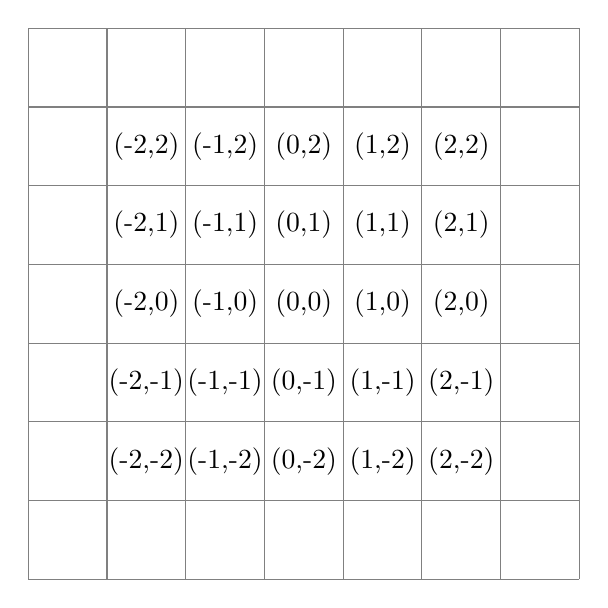
\begin{tikzpicture}
    \draw[step=1.0cm,color=gray] (-4,-4) grid (3,3);
    \node at (-0.5,-0.5) {(0,0)};
    \node at (+0.5,-0.5) {(1,0)};
    \node at (-1.5,-0.5) {(-1,0)};
    \node at (-0.5,+0.5) {(0,1)};
    \node at (-0.5,-1.5) {(0,-1)};
    \node at (+1.5,-0.5) {(2,0)};
    \node at (-2.5,-0.5) {(-2,0)};
    \node at (-0.5,+1.5) {(0,2)};
    \node at (-0.5,-2.5) {(0,-2)};
    \node at (+0.5,+0.5) {(1,1)};
    \node at (-1.5,+0.5) {(-1,1)};
    \node at (+0.5,-1.5) {(1,-1)};
    \node at (-1.5,-1.5) {(-1,-1)};
    \node at (+1.5,+1.5) {(2,2)};
    \node at (-2.5,+1.5) {(-2,2)};
    \node at (+1.5,-2.5) {(2,-2)};
    \node at (-2.5,-2.5) {(-2,-2)};
    \node at (+0.5,+1.5) {(1,2)};
    \node at (-1.5,+1.5) {(-1,2)};
    \node at (+0.5,-2.5) {(1,-2)};
    \node at (-1.5,-2.5) {(-1,-2)};
    \node at (+1.5,+0.5) {(2,1)};
    \node at (-2.5,+0.5) {(-2,1)};
    \node at (+1.5,-1.5) {(2,-1)};
    \node at (-2.5,-1.5) {(-2,-1)};
  \end{tikzpicture}

  \caption{Our naming scheme of squares.}
  \label{fig:grid}

\end{figure}
%%%

\subsection*{Other Cases: $d \neq 0$, $d < \infty$}
So far, we studied the dynamics of the outer billiard system for two particular parameters, which turned out to have simple structures.
For general cases, however, the dyanamics is considerably more complicated.
We show several results of numerical simulations for a particular parameter, $d = 1.0$ (the choice is arbitrary), and make conjectures about properties of the system.
However, we have no proof for any of the claims that we will make.

The orbits of any points in a bounded set seem to be bounded.
Figure~\ref{fig:disk10} is the disk of radius 10 transformed by 500 iterations of the billiard map.
This figure shows that no point escapes to a region far from the origin.
The points remain in a region resembling a square rotated by $\pi/4$.
Note that, since our mapping is a homeomorphism, the region in the figure is homeomorphic to a disk, even though it does not appear so.
\begin{figure}[ht]
  \begin{center}
    \includegraphics[width=0.6\textwidth]{disk10}
    \caption{Left: transformation of an annular region between two circles of radii 1 and 10 after 500 iterations.
      $d = 1.0$.
      Since the billiard map is the identity map for points inside the kite, we can regard this as a transformation of a disk of radius 10.
    }
    \label{fig:disk10}
  \end{center}
\end{figure}

In Figure~\ref{fig:strip2-3}, we see four hollow circles symmetrically placed around the kite.
It is easy to see that these circles are mapped to each other, and in a way similar to the $d \to \infty$ case, form a group of clusters of period $4$.
Unlike the $d \to \infty$ case, however, each point in a periodic cluster may not have the same period.
Also in Figure~\ref{fig:strip2-3}, we see eight clusters of ellipse-like regions; these are 8-periodic clusters.
In the transformations of annular regions of larger radii, we see clusters with higher periods (Figure~\ref{fig:strip3-4-6-7}).
Thus, periodic clusters, which were square-shaped in the $d \to \infty$ case, have various circular shapes.
For $d = 0.1$, Mayer has found periodic clusters of various periods by a numerical simulation (personal communication).
Unlike the $d \to \infty$ case, the periods are not only those of multiples of four, but also multiples of two and odd periods.

\begin{figure}[ht]
  \begin{center}
    $
    \begin{array}{l}
      \includegraphics[width=0.5\textwidth]{strip2-3_setup}
    \end{array}
    $\scalebox{1.75}{$\Rar$}$
    \begin{array}{l}
      \includegraphics[width=0.5\textwidth]{strip2-3}
    \end{array}
    $
    \caption{
      The transformation of an annular region between two circles of radius 2 and 3 after 500 iterations.
      $d = 1.0$.
    }
    \label{fig:strip2-3}
  \end{center}
\end{figure}

\begin{figure}[ht]
  \begin{center}
    \includegraphics[width=0.49\textwidth]{strip3-4}
    \includegraphics[width=0.49\textwidth]{strip6-7}
    \caption{Left: transformation of an annular region between two circles of radii 3 and 4 after 500 iterations.
      Right: between radii 6 and 7.
      $d = 1.0$ for both plots.
    }
    \label{fig:strip3-4-6-7}
  \end{center}
\end{figure}
%%%

When a point is aperiodic, its orbit seems to be sensitive to initial conditions.
Figure~\ref{fig:sensitivity1} shows the evolution of distances between two nearby points.
The points are $(4,\pi/10)$ and a nearby point obtained by rotating the first point by the smallest possible rotation.
Initially, the distance between the two points is essentially zero, and the two points remain close to each other in the beginning.
After around the 500th iteration, however, the distance between the two starts growing.
The growth ends when the distance is around 9, which seems to be the upper bound.
Then, the two points begin to come close to each other again.
The two points keep distance from each other between 1500-3500 iterations, but after the 3500th iteration, the distance between the two oscillates between the upper bound and some small value less than 1.
These two points seem to satisfy the criteria of Li-Yorke pair.
Also, there seem to be uncountably many such points (Figure~\ref{fig:strip2-3},\ref{fig:strip3-4-6-7}).
If these claims are true, then the system is chaotic in the sense of Li-Yorke and also in the sense of Wiggins.

In the periodic clusters, on the other hand, the distance between two nearby points shows almost no growth (Figure~\ref{fig:sensitivity2}).
In this plot, the two points we are looking at are $(4,\pi/4)$ and a nearby point.
Note that the point $(4,\pi/4)$ is in one of the periodic clusters, while $(4,\pi/10)$ is not (Figure~\ref{fig:strip3-4-6-7}).
We do not yet know whether points in periodic clusters are periodic, since it is possible that the set of periodic clusters of the same period is a topologically transitive system.
However, this numerical result suggests that points in periodic clusters are periodic points, as they were in the special case $d \to \infty$.

\begin{figure}[ht]
  \begin{center}
    \includegraphics[width=0.8\textwidth]{billiard_sensitivity_pi-div-10}
    \caption{The evolution of distance between $p = (4, \pi/10)$ and the other point $q$, which is initially close to $p$.
      $q$ was obtained by rotating $p$ by $\epsilon$ radian, where $\epsilon$ is the smallest double available in the precision of the machine.
      The $x$-axis is the number of iterations, and the $y$-axis is the distance between $p$ and $q$.
    }
    \label{fig:sensitivity1}
  \end{center}
\end{figure}
%%%
\begin{figure}[ht]
  \begin{center}
    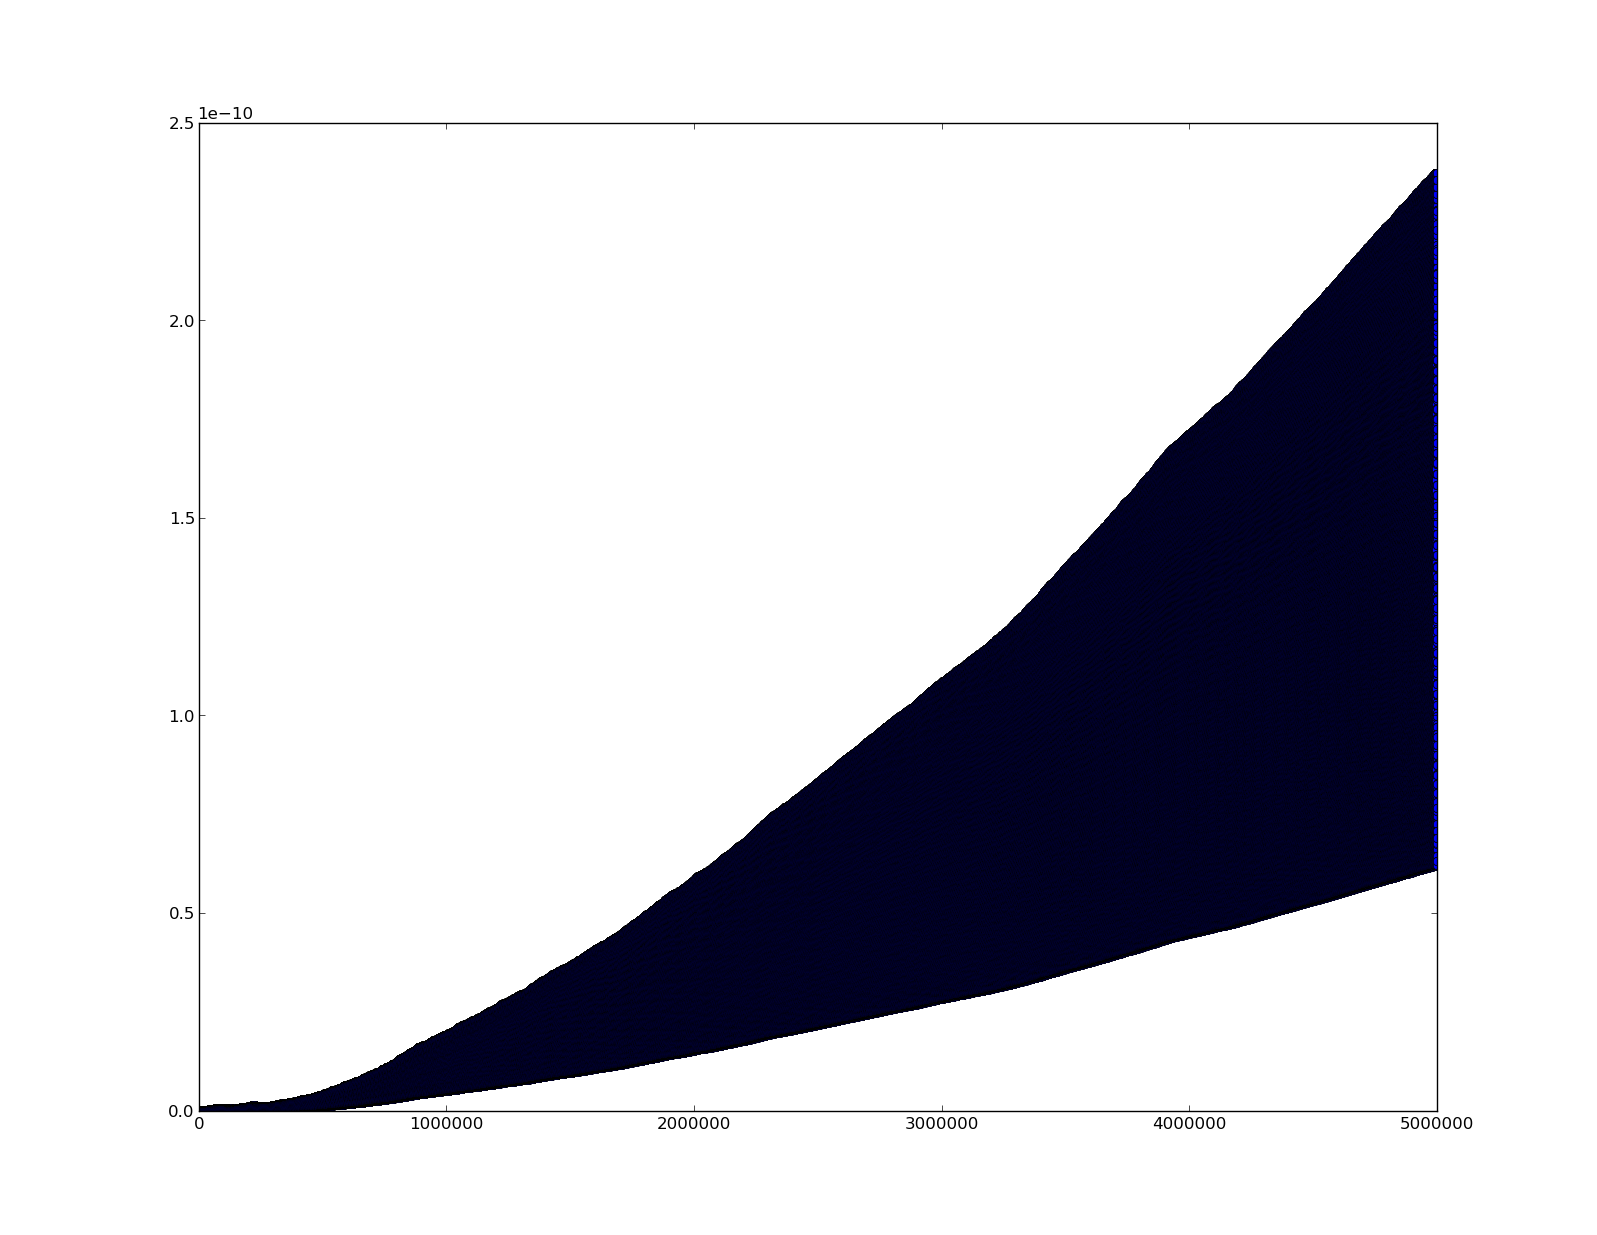
\includegraphics[width=0.8\textwidth]{sensitivity_test_slow_growth_45deg}
    \caption{The evolution of distance between $p = (4, \pi/4)$ and the other point $q$, which is initially close to $p$.
      $q$ was obtained by rotating $p$ by $\epsilon$ radian, where $\epsilon$ is the smallest double available in the precision of the machine.
      The $x$-axis is the number of iterations, and the $y$-axis is the distance between $p$ and $q$.
      Even after $5.0 \times 10^6$ iterations, the distance between the two points is on the order of $10^{-1}$.
    }
    \label{fig:sensitivity2}
  \end{center}
\end{figure}

\bibliographystyle{../../bibliography/pjgsm}
\bibliography{../../bibliography/thesis}

\printindex
\end{document}


